\documentclass[%
 reprint,
%superscriptaddress,
%groupedaddress,
%unsortedaddress,
%runinaddress,
%frontmatterverbose, 
%preprint,
%preprintnumbers,
%nofootinbib,
%nobibnotes,
%bibnotes,
 amsmath,amssymb,
 aps,
%pra,
%prb,
%rmp,
%prstab,
%prstper,
%floatfix,
]{revtex4-2}

\usepackage{graphicx}% Include figure files
\usepackage{dcolumn}% Align table columns on decimal point
\usepackage{bm}% bold math
\usepackage{physics}
\usepackage{cancel}
\usepackage{float}
%\usepackage{hyperref}% add hypertext capabilities
%\usepackage[mathlines]{lineno}% Enable numbering of text and display math
%\linenumbers\relax % Commence numbering lines

%\usepackage[showframe,%Uncomment any one of the following lines to test 
%%scale=0.7, marginratio={1:1, 2:3}, ignoreall,% default settings
%%text={7in,10in},centering,
%%margin=1.5in,
%%total={6.5in,8.75in}, top=1.2in, left=0.9in, includefoot,
%%height=10in,a5paper,hmargin={3cm,0.8in},
%]{geometry}

\begin{document}

\preprint{APS/123-QED}

\title{Stability Regime of Spheromak m=1 Tilt Mode}% Force line breaks with \\

\author{Evan Bluhm}
%  \altaffiliation[Also at ]{Physics Department, XYZ University.}%Lines break automatically or can be forced with \\
% \author{Second Author}%
%  \email{Second.Author@institution.edu}
% \affiliation{%
%  Authors' institution and/or address\\
%  This line break forced with \textbackslash\textbackslash
% }%


\date{May 28, 2021}% It is always \today, today,
             %  but any date may be explicitly specified
\begin{abstract}

The stability of the force-free axisymmetric spheromak configuration was investigated by linearizing the ideal magnetohydrodynamic (MHD) equations about a static equilibrium. The linearized MHD equations were integrated in time using a finite difference method, subject to rigid conducting wall boundary conditions. The static spheromak equilibrium was expected to be stable for elongation ratio $L/R < 1.67$.  Instead, unstable modes were observed for all values of $L/R$, indicating numerical instability in the finite difference method applied.

% % \begin{description}
% % \item[Usage]
% % Secondary publications and information retrieval purposes.
% % \item[Structure]
% % You may use the \texttt{description} environment to structure your abstract;
% % use the optional argument of the \verb+\item+ command to give the category of each item. 
% % \end{description}
\end{abstract}

%\keywords{Suggested keywords}%Use showkeys class option if keyword
                              %display desired
\maketitle

%\tableofcontents

\section{Linearized Ideal MHD}

To investigate the stability of a configuration which is initially force-free, it is useful to linearize the equations of ideal MHD about a static equilibrium. Doing so allows us to calculate the growth rates of Fourier modes, thereby exploring the states which are stable or unstable. If there are any modes which grow in time, then the configuration is unstable.

We consider an initial static equilibrium, defined by $\rho_0$, $\vec v_0$, $\vec B_0$, and $p_0$, such that $\vec v_0 = 0$. If we add a small perturbation $\rho_1$, $\vec v_1$, $\vec B_1$, $p_1$ on top of the equilibrium, we would like to know how the perturbation will evolve in time. Plugging the sum of the initial perturbation and equilibrium into the nonlinear MHD equations, and discarding all quantities of order greater than 1 in a perturbation term, we arrive at the linearized ideal MHD equations:

\begin{equation}
\pdv{\rho_1}{t} = - \div ( \rho_0 \vec v_1)    
\end{equation}
\begin{equation}
\pdv{p_1}{t} = - \div (p_0 \vec v _1) + (1 - \gamma) p_0 \div \vec v_1 
\end{equation}
\begin{equation}
\pdv{\vec B_1}{t} = \curl ( \vec v_1 \cross \vec B_0)
\end{equation}
\begin{equation}
\rho_0 \pdv{\vec v_1}{t} = \grad p_1 + \frac{1}{\mu_0} \left[ (\curl \vec B_1) \cross \vec B_0 + (\curl \vec B_0) \cross \vec B_1 \right]
\end{equation}

Note that the density equation has de-coupled from the others, such that we may evolve the perturbed velocity, magnetic field, and pressure in time without the need to evolve the density.

From here onwards, we will use the following notation for the equilibrium and perturbation terms, to simplify the number of indices required for finite difference expressions:
\begin{equation}
\vec B \equiv \vec B \qquad  \vec b \equiv \vec B_1
\end{equation}
\begin{equation}
\vec v_1 = u \vu r + v \vu \theta + w \vu z
\end{equation}

We use a finite difference method to integrate the linearized MHD equations in time and determine the evolution of the perturbation. The equilibrium quantities $\vec B$, $\vec p_0$, $\vec \rho_0$ remain static in time, while we integrate the perturbed quantities over a discrete grid.

Here, we investigate the stability properties of an axisymmetric force-free spheromak configuration, as described in Section IV. For an axisymmetric configuration, we only require a two-dimensional spatial grid, such that $r = j \Delta r$ and $z = k \Delta z$). We also discretize time by $t = n \Delta t$. We replace the continuous perturbation by sampled values on the grid:
\begin{equation}
u(r, z, t) = u_{j, k} ^{n}
\end{equation}

By forming finite difference expressions for the derivatives in the linearized ideal MHD equations, we arrive at a finite difference system of the form
\begin{eqnarray}
{p_1}_{jk} ^{n+1} &=& {p_1}_{ij} ^n + \Delta t \left[ \ldots \right]^n \\
{\vec b}_{jk} ^{n+1} & = & {\vec{b}}_{jk} ^n + \Delta t [ \ldots ] ^n \\
{\vec v} _{jk} ^{n+1} & = & {\vec v}_{jk} ^{n+1} + \Delta t [\ldots ]^n
\end{eqnarray}
These expressions evolve the perturbation across the entire grid by $\Delta t$ in an explicit, iterative manner. The finite difference expressions are computed in Appendix A.

\section{Boundary Conditions}

With the time-dependent evolution and initial conditions specified, boundary conditions are also required to integrate the linearized ideal MHD equations in time. In our spheromak configuration, we have three separate boundaries to consider: the conducting wall at $r=R$, the conducting caps at $z=[0, L]$, and the z-axis itself at $r=0$.

At the conducting wall boundary $r = R$ ($j=M_r$), we impose $\vec v \cdot \vu r = 0$ and $\vec b \cdot \vu r = 0$. The condition on the magnetic field at the conducting boundary is actually $\pdv{}{t} \vec b \cdot \vu r = 0$. Our equilibrium and initial perturbed fields both satisfy $b_r(r=R) = 0$ by construction. In order to alter our finite difference expressions at the $r = R$ boundary, we also need a finite difference expression for $\pdv{u}{r}$ that does not use points outside the domain. At the boundary, we use a one-sided first-order difference
\begin{equation}
\left. \pdv{u}{r} \right|_{r = R} \approx \frac{u_{M_r, k} - u_{M_r-1, k}}{\Delta r}
\end{equation}
Applying these conditions at the boundary, we have the modified finite difference expressions. Where not otherwise specified, the spatial indexes are $M_r, k$:
\begin{equation}
{b_r}_{M_r, k} ^{n+1} = 0 \qquad {v_r}_{M_r, k} ^{n+1} = 0
\end{equation}
\begin{eqnarray*}
{b_\theta} _{M_r, k} ^{n+1} = {b_\theta}_{M_r, k} ^{n} + \Delta t \left[ - w \pdv{B_\theta}{z} + v \left( \pdv{B_z}{z} + \pdv{B_r}{r} \right) \right. \\
\left.  + i m B_z v - B_\theta \frac{w_{M_r, k+1}- w_{M_r, k-1}}{2 \Delta z} + B_r \frac{u_{M_r, k} - u_{M_r-1, k}}{\Delta r} \right] \\
\end{eqnarray*}
\begin{eqnarray*}
{b_z}_{M_r, k} ^{n+1} = {b_z}_{M_r, k} ^{n} + \frac{\Delta t}{r} \left[B_\theta i m w + w (B_r + r \pdv{B_r}{r}) \right. \\
\left. - B_z\left(i m v + r \frac{u_{M_r, k}-u_{M_r-1, k}}{\Delta r} \right) + r B_\theta \frac{w_{M_r, k}-w_{M_r-1, k}}{\Delta r} \right] \label{bc-bz-r}
\end{eqnarray*}
\begin{eqnarray*}
v_{M_r, k} ^{n+1} = v_{M_r, k} ^{n} + \frac{\Delta t}{r \mu_0 \rho_0} \left[ b_z r \pdv{B_\theta}{z} + r B_r \frac{{b_\theta}_{M_r, k} - {b_\theta}_{M_r-1, k}}{\Delta r} \right. \\
\left. + B_r b_\theta  + B_z \left( r \frac{{b_\theta}_{M_r, k+1} - {b_\theta}_{M_r, k-1}}{2 \Delta z} - i m b_z \right) \right]
\end{eqnarray*}
\begin{eqnarray*}
w_{M_r, k} ^{n+1} = w_{M_r, k} ^n + \frac{\Delta t}{\rho_0 \mu_0 r} \left[  r B_r \frac{{b_z}_{M_r, k} - {b_z}_{M_r - 1, k}}{\Delta r} \right. \\
\left. + B_\theta \left( - r \frac{{b_\theta}_{M_r, k+1} - {b_\theta}_{M_r, k-1}}{2 \Delta z} + i m b_z \right) - b_\theta r \pdv{B_\theta}{z} \right]
\end{eqnarray*}

We treat the rigid conducting boundaries at $z=0$ and $z=L$ in the same manner.

The boundary at $r=0$ also requires special treatment. We are performing a modal analysis of $m=1$ Fourier modes of the form $g_1(r, \theta, z, t) = g_1(r, z, t) e^{i m \theta}$. To obtain consistent, analytic solutions, the perturbed quantities must satisfy the following conditions at the axis:
\begin{equation}
b_\theta = i b_r \qquad b_z = 0 \qquad v = i u \qquad w = 0
\end{equation}
\begin{equation}
\pdv{u}{r} = \pdv{v}{r} = \pdv{b_r}{r} = \pdv{b_\theta}{r} = 0
\end{equation}
With these conditions, we can replace instances of the normal components of the vector fields and their derivatives, but we are left with several singularities of the form
\begin{equation}
\lim_{r \rightarrow 0} \frac{1}{r} \pdv{w}{\theta}
\end{equation}
For quantities which go to zero as $r \rightarrow 0$, we can form the limit as:
\begin{eqnarray}
\lim_{r \rightarrow 0} \frac{1}{r} \pdv{w}{\theta} & = & \lim_{r \rightarrow 0} \frac{i m w}{r} \\
& = & \pdv{(i m w)}{r} / \pdv{r}{r} \\
& = & i m \pdv{w}{r}
\end{eqnarray}
We also require a one-sided finite difference to compute the radial derivative at the axis:
\begin{equation}
\left. \pdv{b_z}{r} \right|_{r=0} \approx \frac{{b_z}_{1, k}-{b_z}_{0,k}}{\Delta r}
\end{equation}
we arrive at the modified finite differences at the $r=0$ boundary:
\begin{eqnarray*}
{b_r}_{0, k} ^{n+1} = {b_r}_{0, k} ^n + \Delta t \left[ B_z \frac{u_{0, k+1}-u_{0, k-1}}{2 \Delta z} + u \pdv{B_z}{z} \right]
\end{eqnarray*}
\begin{eqnarray*}
{b_\theta}_{0, k} ^{n+1} = {b_\theta}_{0, k} ^{n} + \Delta t \left[ i m B_z v + v \left( \pdv{B_z}{z} + \pdv{B_r}{r} \right) - u \pdv{B_\theta}{r} \right]
\end{eqnarray*}
\begin{eqnarray*}
u_{0, k} ^{n+1} = u_{0, k} ^n + \frac{\Delta t}{\mu_0 \rho_0} \left[ - b_\theta \pdv{B_\theta}{r} \right. \\ 
\left. + B_z \left( \frac{{b_r}_{0, k+1}-{b_r}_{0, k-1}}{2 \Delta z} - \frac{{b_z}_{1, k}}{\Delta r} \right) \right]
\end{eqnarray*}
\begin{eqnarray*}
v_{0, k} ^{n+1} = v_{0, k} ^n + \frac{\Delta t}{\mu_0 \rho_0} \left[ B_z \pdv{b_\theta}{z} + b_r \pdv{B_\theta}{r} \right]
\end{eqnarray*}

\section{Spheromak Equilibrium}

In this paper, we wish to evaluate the stability criteria for the axisymmetric force-free spheromak configuration, as given in Reference \cite{BondesonA1981Tioa}:

\begin{eqnarray}
B_r & = & - k_z J_1(k_r r) \cos (k_z z) \label{spheromak-eqn-start}\\
B_\theta & = & \lambda_0 J_1(k_r  r) \sin (k_z z) \\
B_z & = & k_r J_0(k_r r) \sin (k_z z) \label{spheromak-eqn-end}
\end{eqnarray}

In particular, we wish to evaluate the stability of the $m=1$ Fourier modes, so our perturbation quantities will be of the form:
\begin{equation}
\vec v(r, \theta, z, t) = \vec v(r, z, t) e^{i \theta}
\end{equation}
\begin{equation}
\vec b(r, \theta, z, t) = \vec b(r, z, t) e^{i \theta}
\end{equation}

Since our configuration is axisymmetric, we can expect the radial dependence of the eigenmodes to be proportional to Bessel functions. When choosing an initial perturbation, we wish to excite as many modes as possible, so we choose an initial perturbation which is sinusoidal in $r$:
\begin{equation}
\vec v_1 = \delta \sin(\pi r/R) \cos (\pi z /L) \vu r \label{spheromak-initial-perturb}
\end{equation}
where $\delta$ is a small perturbation. 

\begin{figure}
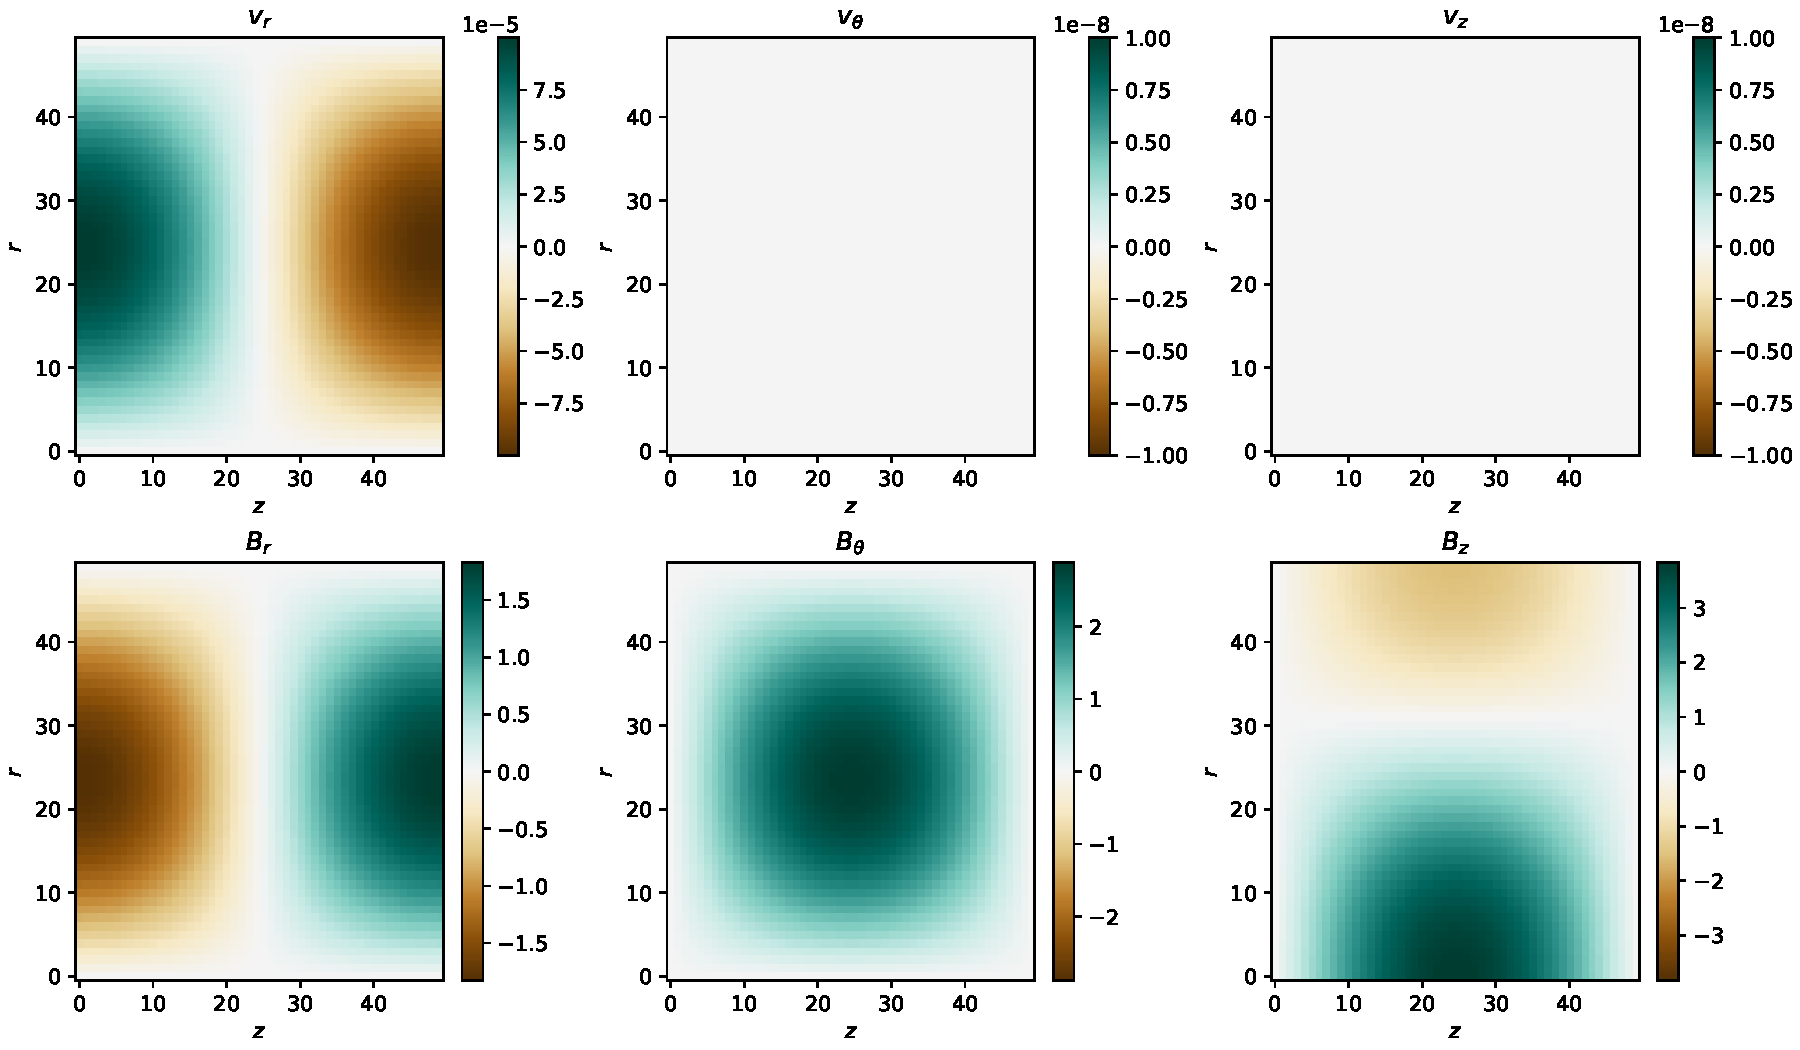
\includegraphics[width=\linewidth]{proj2-3/spheromak_initial_config.pdf}
\caption{\label{fig:spheromak-initial-conditions}Un-normalized initial conditions for our linear MHD solver. The top three plots show a small radial perturbation in velocity which meets the boundary conditions, as given by equation \ref{spheromak-initial-perturb}. The bottom three plots show the equilibrium $\vec B_0$ given by equations \ref{spheromak-eqn-start}-\ref{spheromak-eqn-end}. }
\end{figure}

\section{Results}

The spheromak equilibrium investigated in this paper is known to be stable to m=1 modes, under the condition $L/R < 1.67$. Our finite difference integrator was unable to reproduce this region of stability. For any value of $L/R$, we observed exponential growth of perturbation modes. This indicates that the instability we observe is due to the numerical method, rather than being a characteristic of the physical system under study.

One possible cause of the growth in numerical errors is a violation of the stability condition for the numerical method itself. In order to accurately capture the wave characteristics, the time step must satisfy the CFL condition
\begin{equation}
\frac{c \Delta t}{\Delta r}
\end{equation}
where $c$ is the largest characteristic speed expected. It is the larger of the sound speed $\sqrt{\gamma p^\star / \rho^\star}$ and the Alfvén speed $\sqrt{{B^\star}^2 / \mu_0 \rho ^\star}$, where $p^\star$ is the maximum of the equilibrium pressure, $\rho^\star$ is the maximum equilibrium density, and $B^\star$ is the maximum magnitude of the equilibrium magnetic field. We have attempted decreasing the time step all the way to $10^{-7}$, and found the same oscillatory errors.

An attempt was made to subdue the oscillatory errors by introducing an artificial diffusion term to the linearized partial differential equation:
\begin{equation}
\pdv{\vec v}{t} = [\ldots] + \sigma \nabla ^2 \vec v
\end{equation}
for small values of $\sigma$. The results of this artificial diffusion term are shown in Figure \ref{fig:spheromak-instability-snapshots-diffusion}. While the errors are no longer oscillatory in nature, the errors continue to grow exponentially in time. Since the errors arise from oscillations near the axis of symmetry, we conclude that the boundary condition at $r = 0$ has not been accurately captured by our finite difference expressions. Further investigation is required to determine appropriate axisymmetric boundary conditions for our system.


\pagebreak 

\begin{figure}[H]
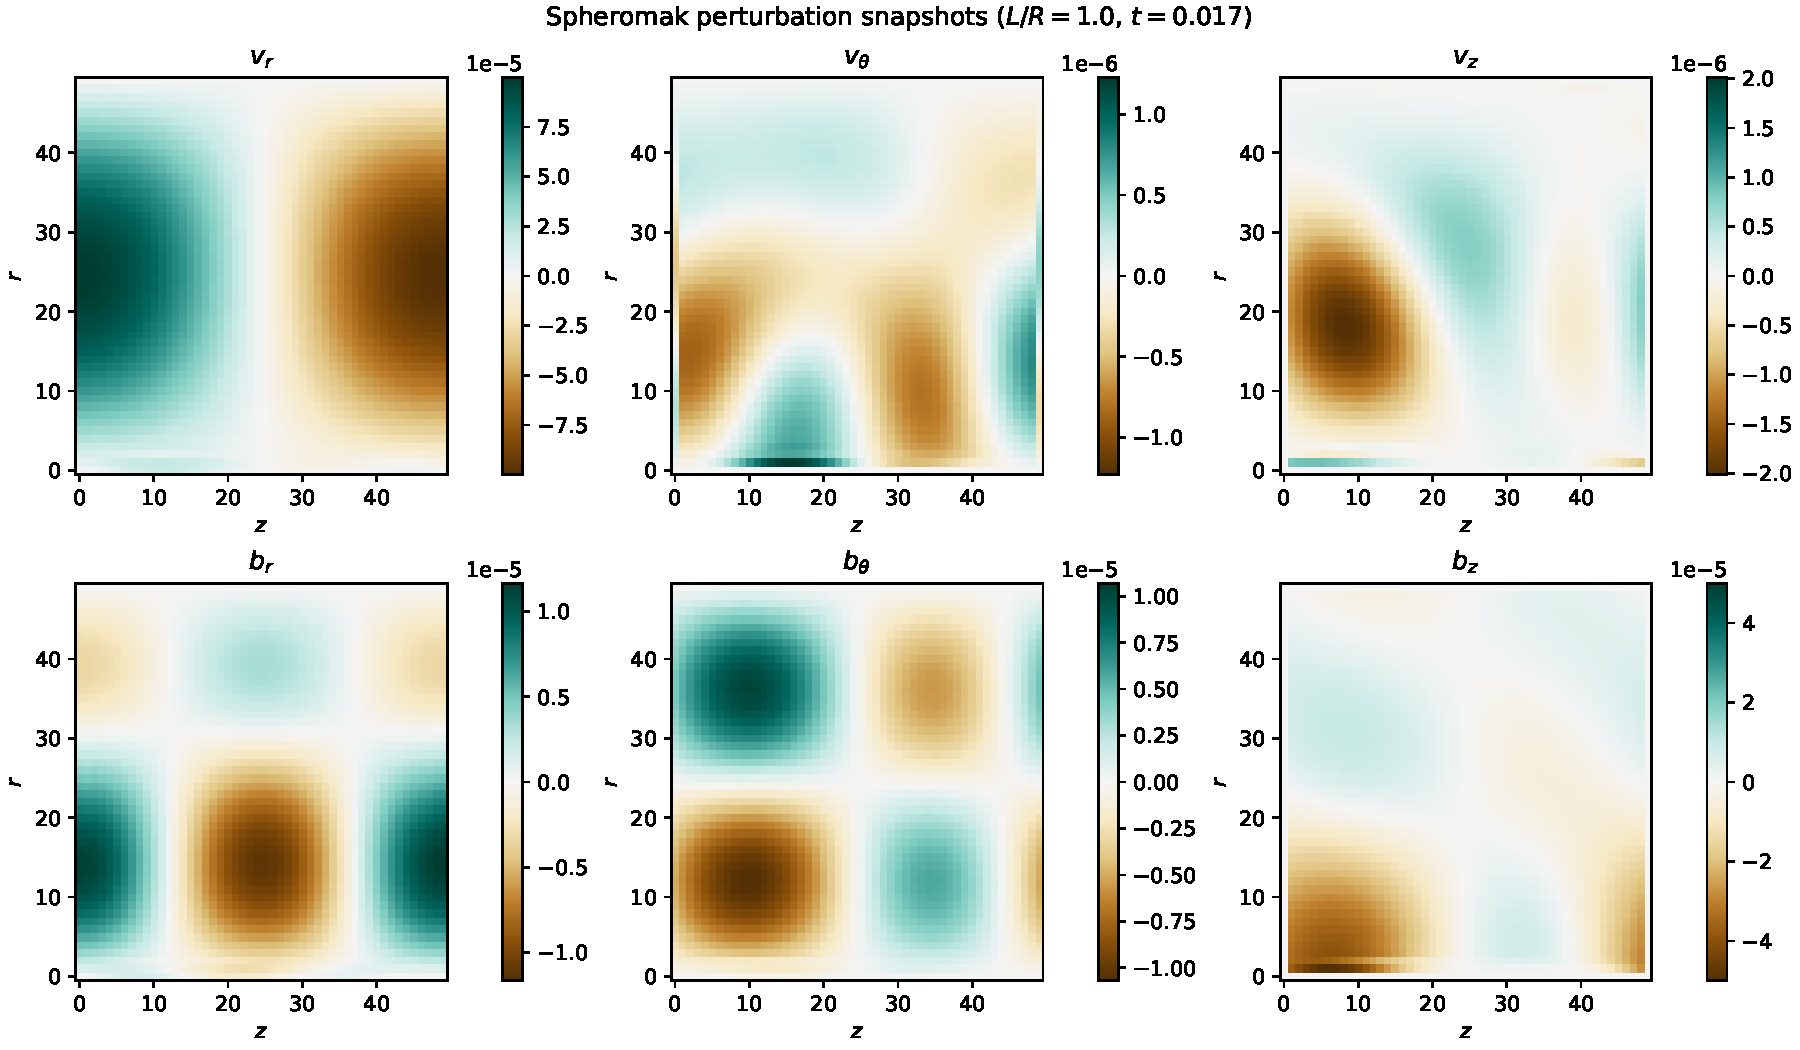
\includegraphics[width=0.9\linewidth]{proj2-3/spheromak_snapshot_1.pdf}
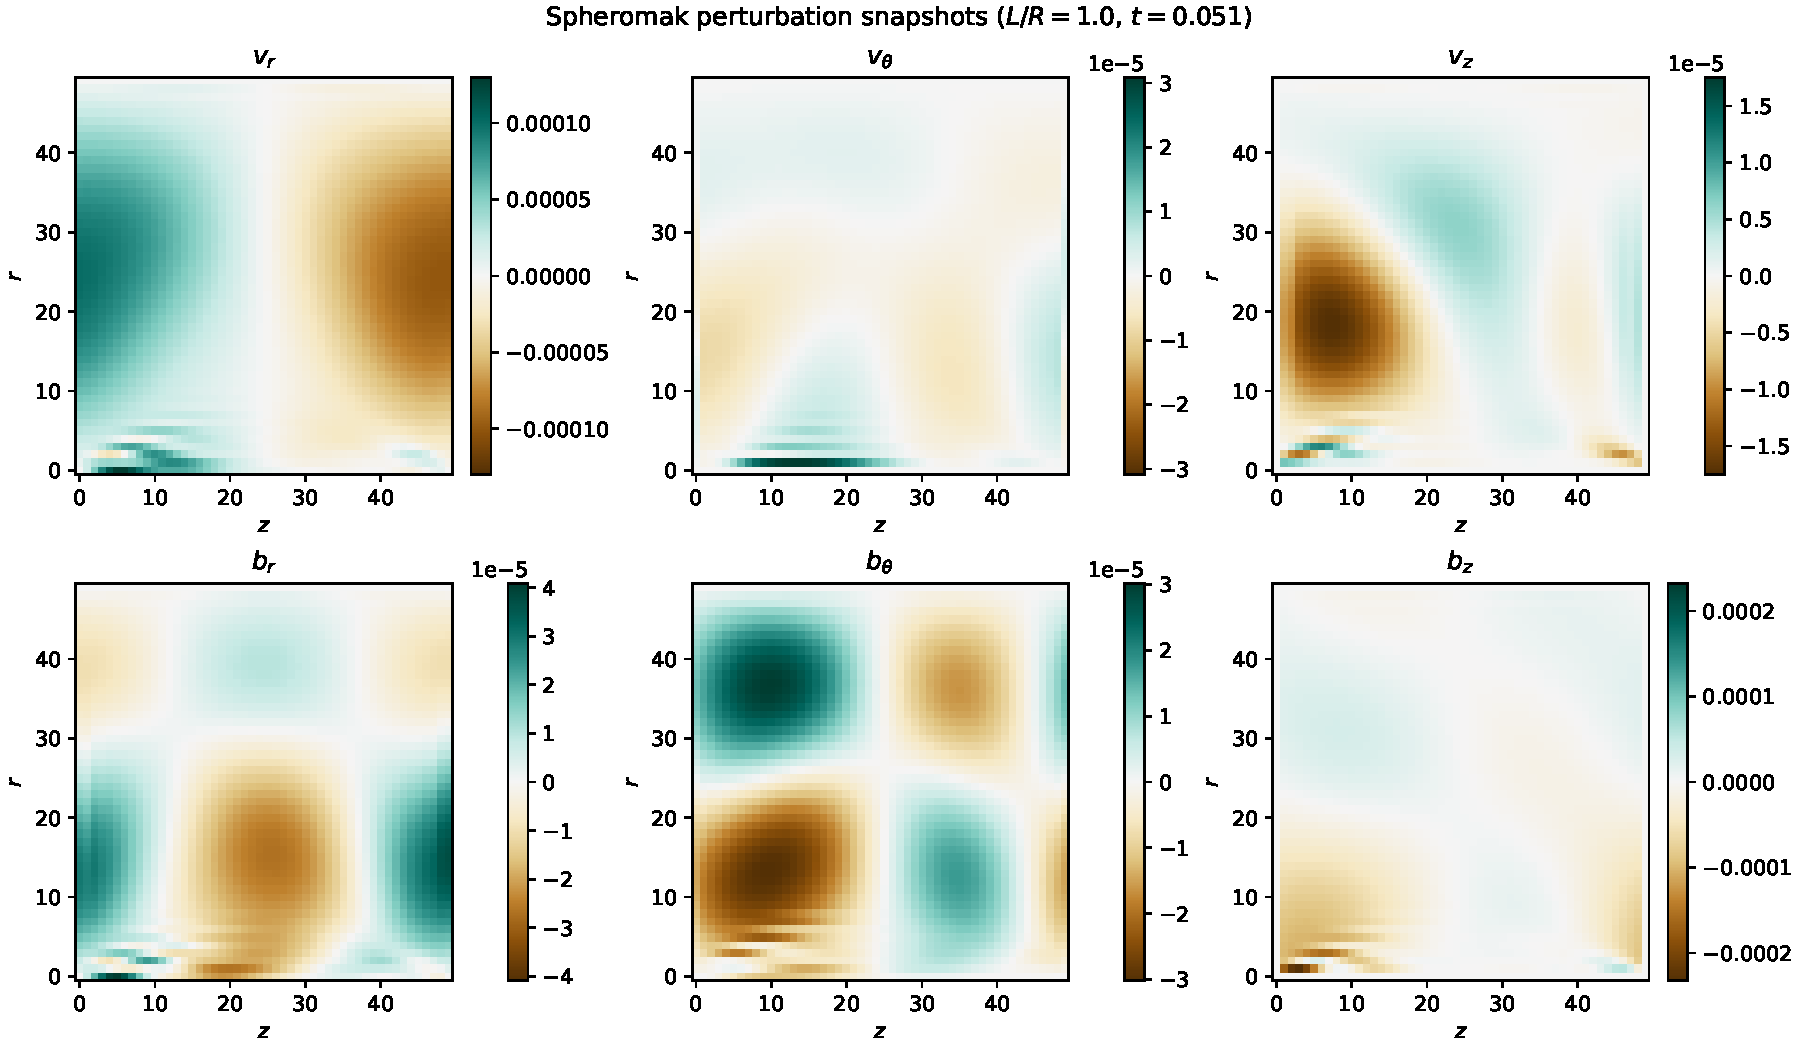
\includegraphics[width=0.9\linewidth]{proj2-3/spheromak_snapshot_3.pdf}
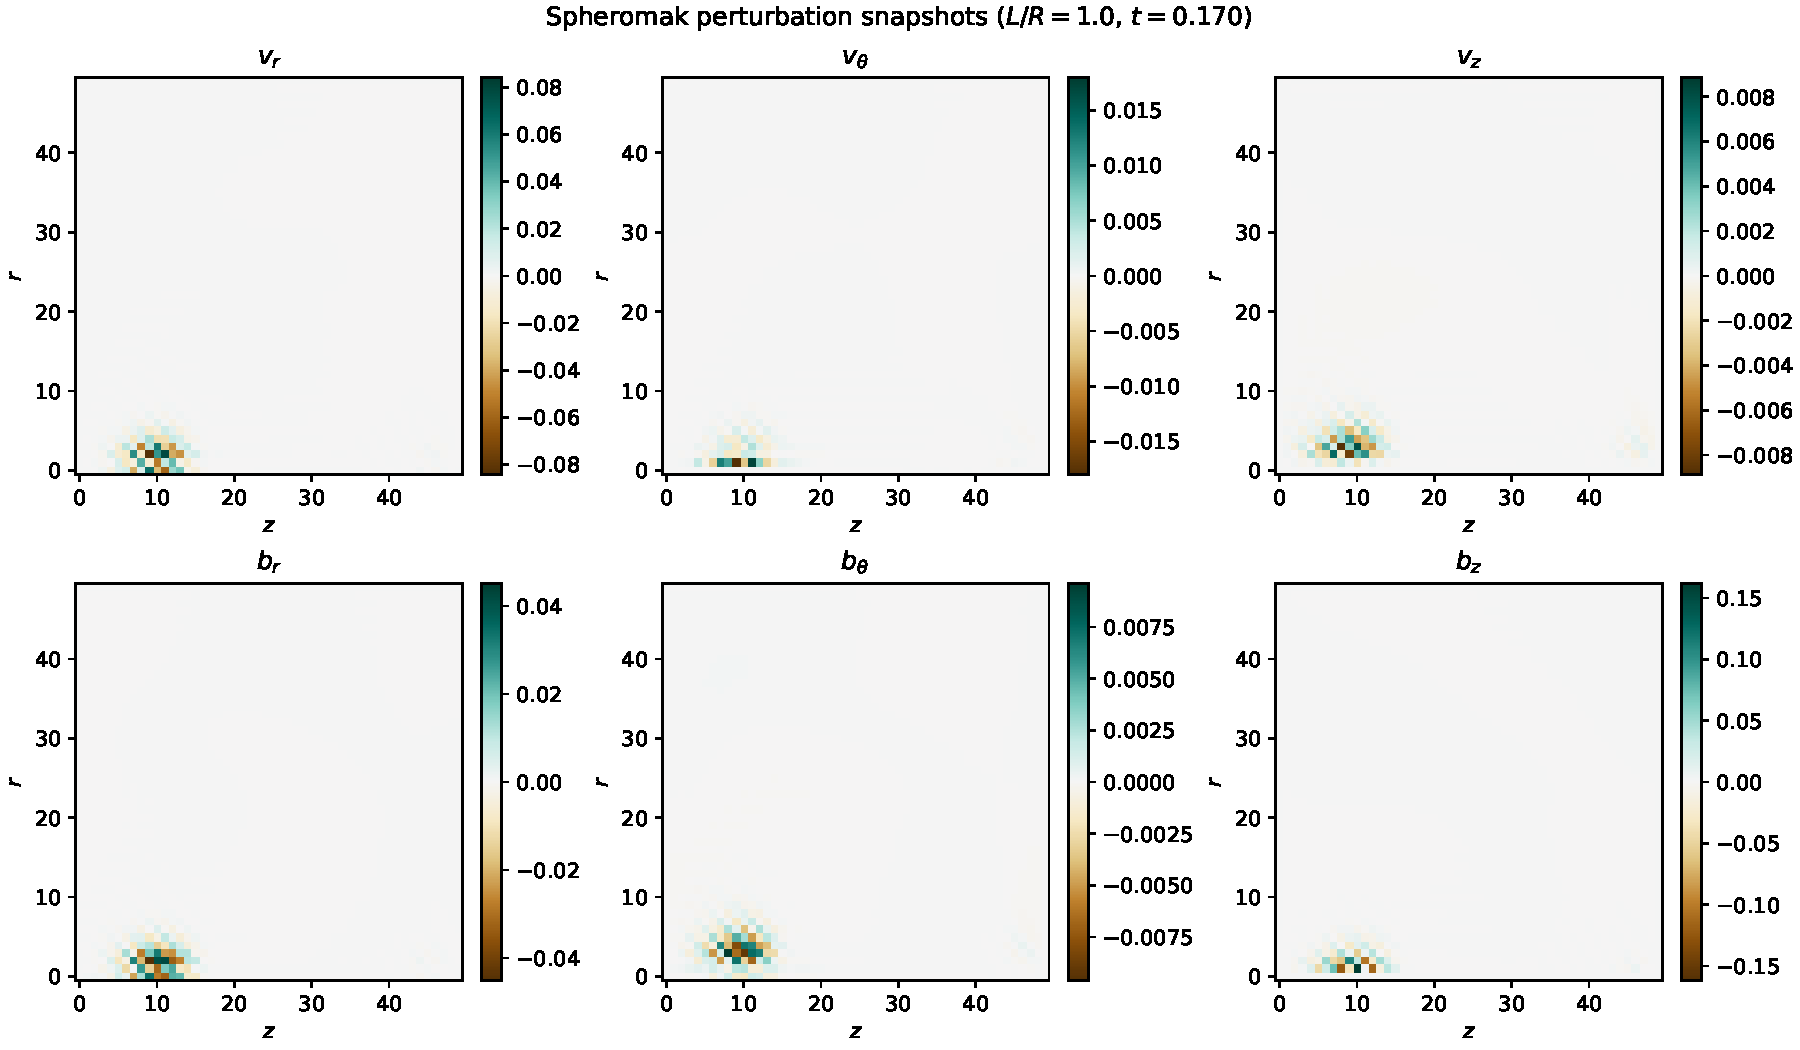
\includegraphics[width=0.9\linewidth]{proj2-3/spheromak_snapshot_10.pdf}
\caption{\label{fig:spheromak-instability-snapshots}Snapshots of the perturbation solution in time, for the initial conditions shown in Figure \ref{fig:spheromak-initial-conditions}. The model parameters are $M_r=50$, $M_z=50$, $\delta =0.0001$, $\Delta t=0.001$, and $L/R=1.0$. These snapshots show the growth of a numerical instability in time near the axis of symmetry. Stationary errors begin to grow, until they dominate the solution by $t=0.1$.}
\end{figure}

\begin{figure}[H]
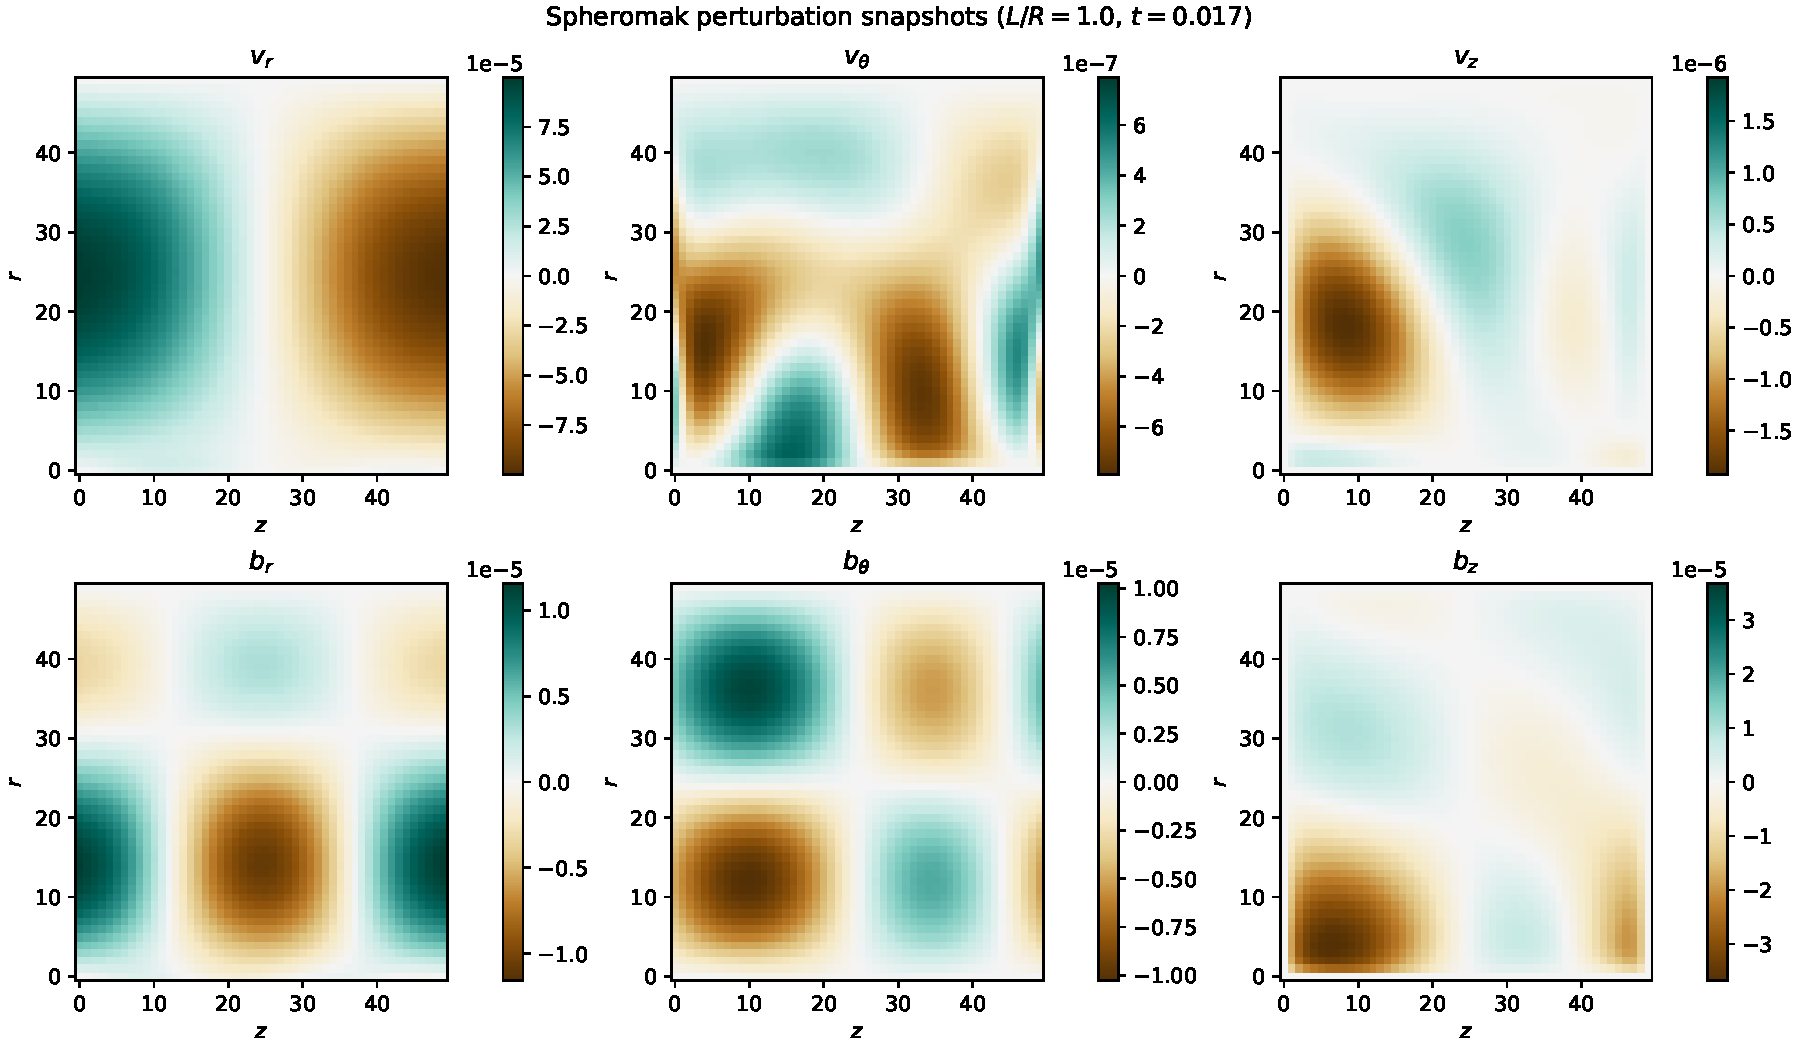
\includegraphics[width=0.9\linewidth]{proj2-3/spheromak_snapshot_diffusion_1.pdf}
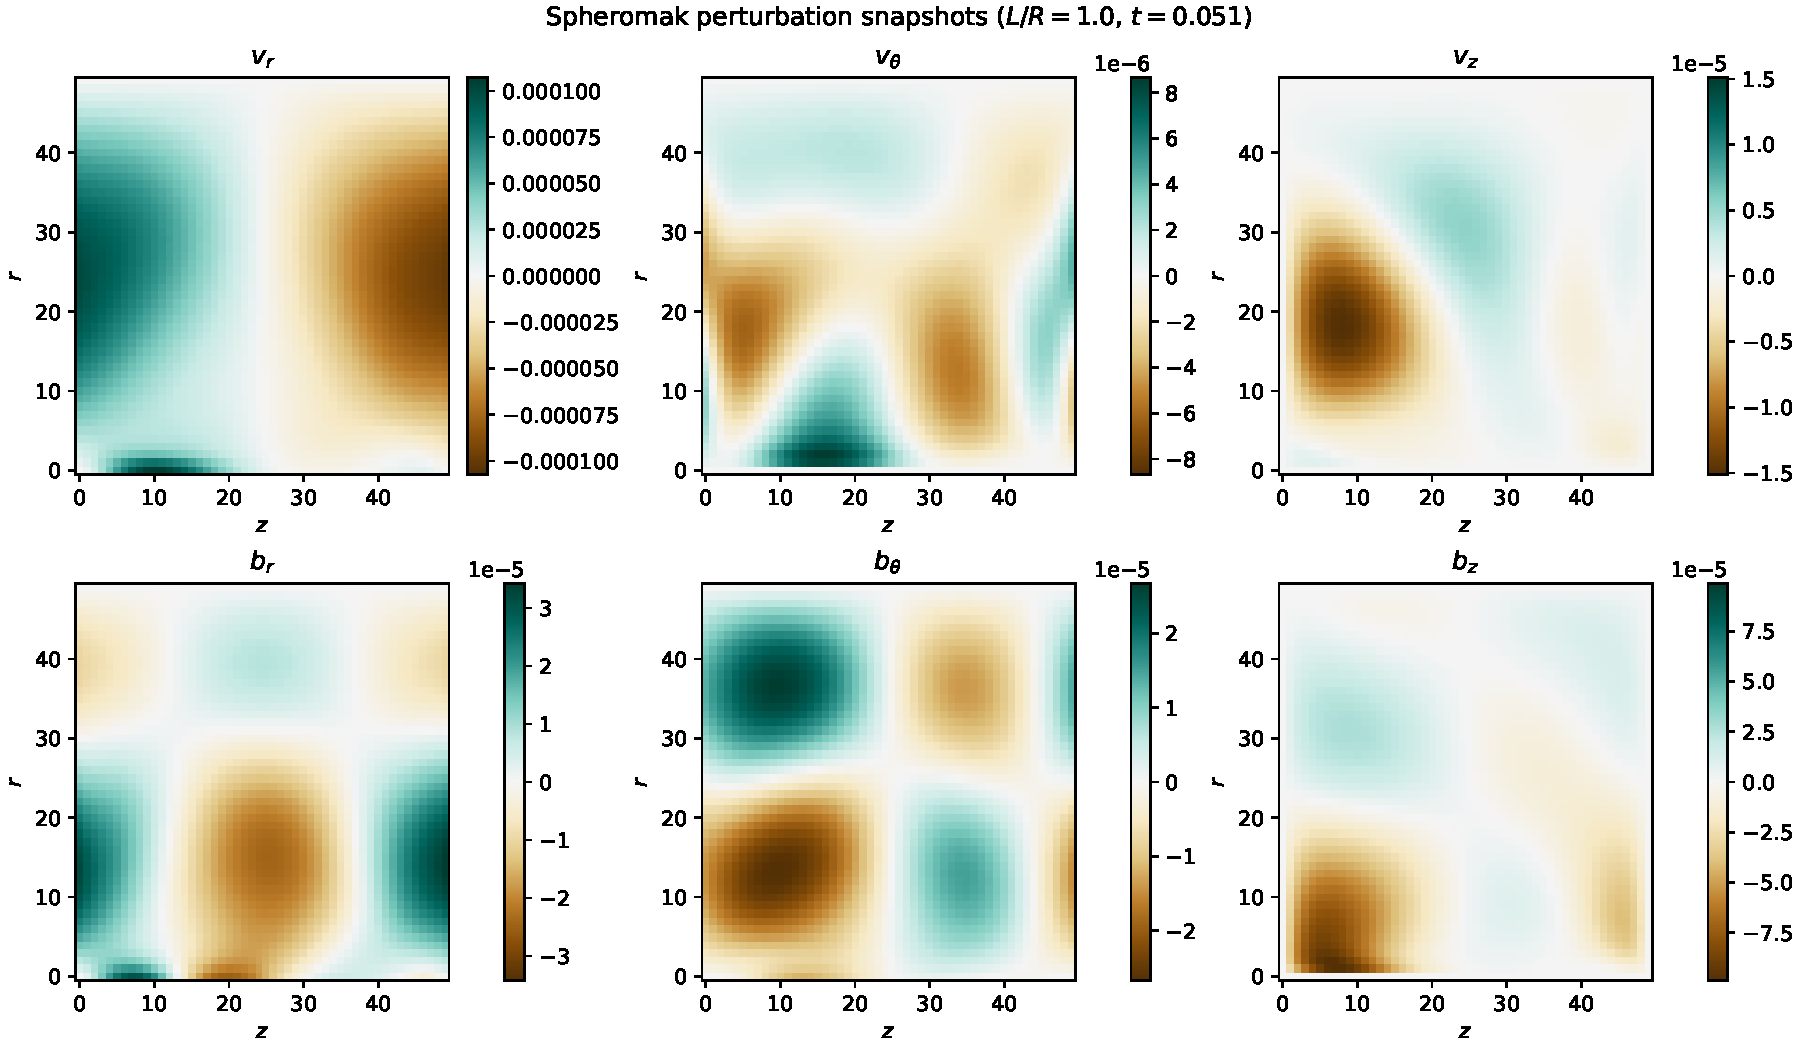
\includegraphics[width=0.9\linewidth]{proj2-3/spheromak_snapshot_diffusion_3.pdf}
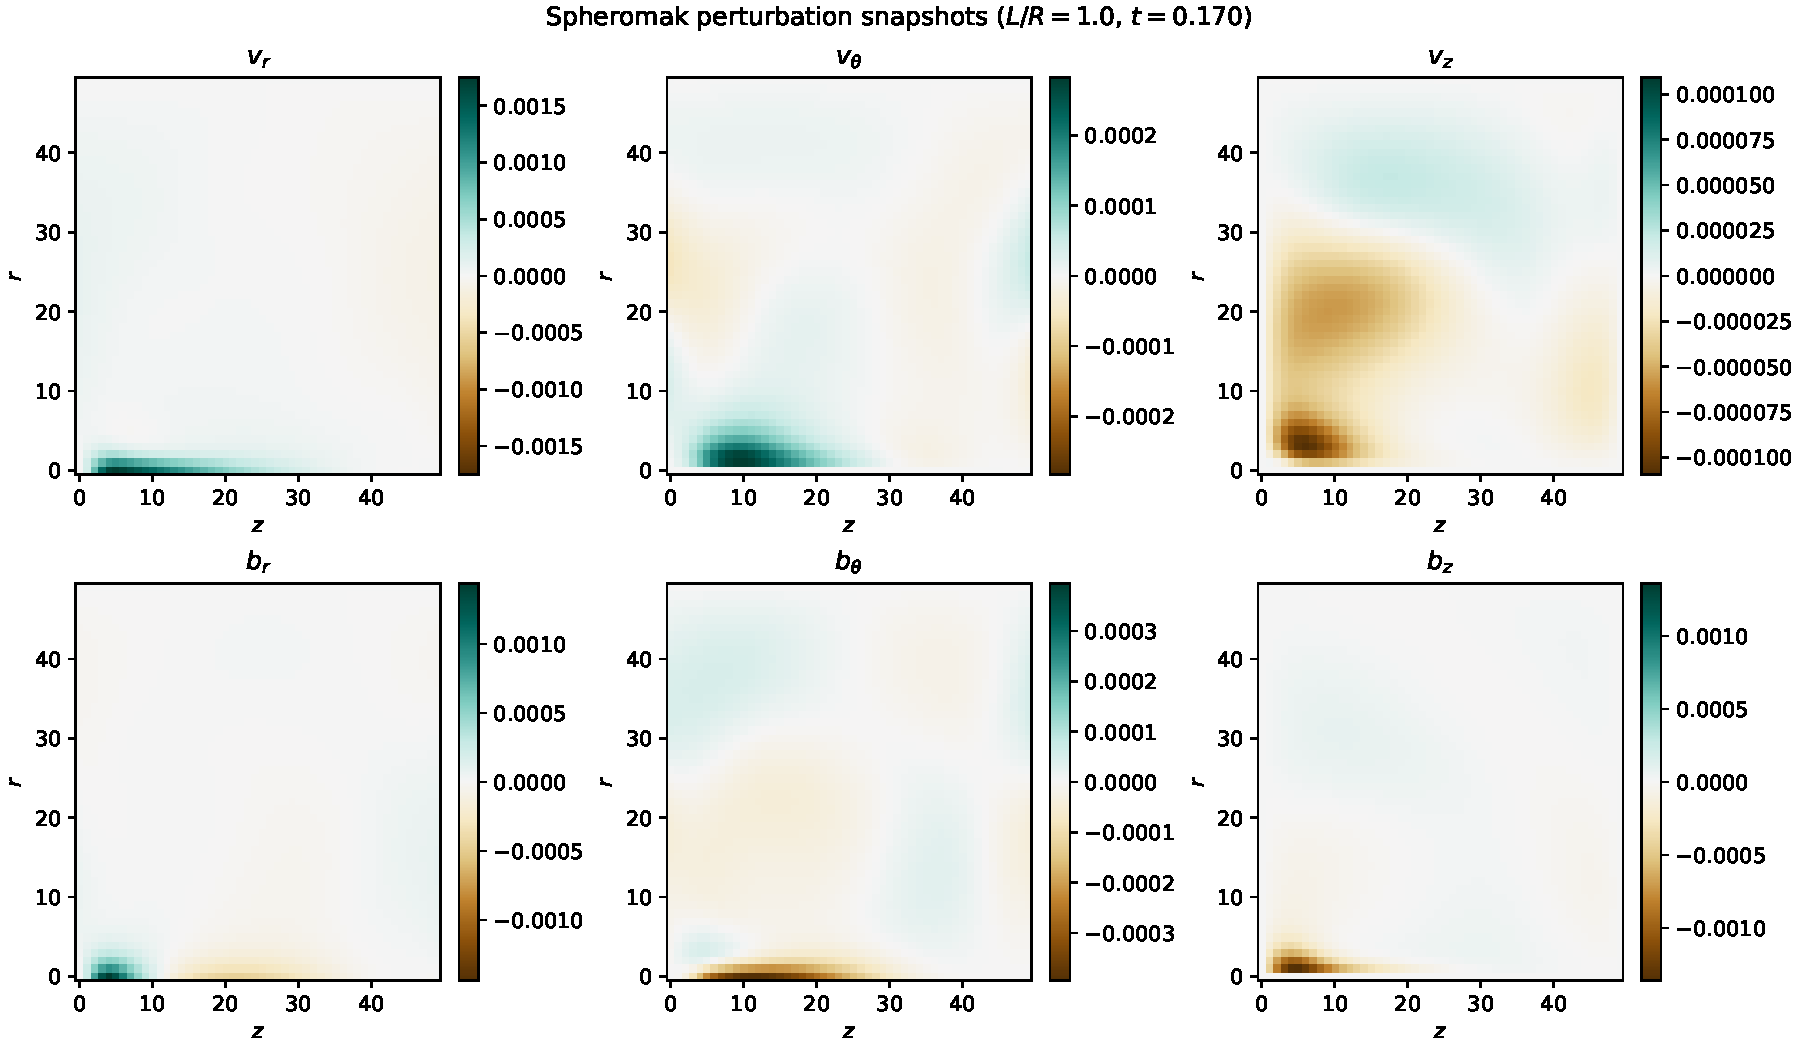
\includegraphics[width=0.9\linewidth]{proj2-3/spheromak_snapshot_diffusion_10.pdf}
\caption{\label{fig:spheromak-instability-snapshots-diffusion}Attempt to resolve numerical instabilities shown in Figure \ref{fig:spheromak-instability-snapshots} by adding a small artificial diffusion term $\sigma \nabla ^2 \vec v$. The shapshots show the result for $\sigma \Delta t / \Delta r ^2 = 0.1$. The errors are no longer oscillatory, but the errors still grow exponentially in time.}
\end{figure}




\nocite{*}

\bibliography{proj2-3}% Produces the bibliography via BibTeX.


\onecolumngrid

\pagebreak

\appendix

\section{Finite Difference Solution of Time-Dependent Linear MHD Equations}

For a static equilibrium $\rho_0, \vec v _0, \vec B_0, p_0$ with a small perturbation $\rho_1(t), \vec v_1(t), \vec B_1(t), p_1(t)$, we discard terms which are second-order in perturbation quantities. The resulting linearized ideal MHD equations for a static equilibrium ($\vec v_0 = 0$) are:

\begin{equation}
\pdv{\rho_1}{t} = - \div ( \rho_0 \vec v_1)    
\end{equation}
\begin{equation}
\pdv{p_1}{t} = - \div (p_0 \vec v _1) + (1 - \gamma) p_0 \div \vec v_1 
\end{equation}
\begin{equation}
\pdv{\vec B_1}{t} = \curl ( \vec v_1 \cross \vec B_0)
\end{equation}
\begin{equation}
\rho_0 \pdv{\vec v_1}{t} = \grad p_1 + \frac{1}{\mu_0} \left[ (\curl \vec B_1) \cross \vec B_0 + (\curl \vec B_0) \cross \vec B_1 \right]
\end{equation}

For a cylindrical equilibrium, we assume angular dependence of the perturbation is:
\begin{equation}
g_1 (r, \theta, z, t) = g_1(r, z, t) e^{i m \theta}
\end{equation}
\begin{equation}
\text{Re}(g_1) = g_1(r, \theta=0, z, t)
\end{equation}
\begin{equation}
\text{Im}(g_1) = g_1(r, \theta=- m \pi/2, z, t)
\end{equation}
such that
\begin{equation}
\pdv{g_1}{\theta} = i m g_1
\end{equation}

For the purposes of our model, we will also limit ourselves to equilibria with:
\begin{equation}
\grad p_0 = 0
\end{equation}
\begin{equation}
\grad \rho_0 = 0
\end{equation}
\begin{equation}
\pdv{\vec B_0}{\theta} = 0
\end{equation}

To make the notation a bit easier to read, let
\begin{equation}
\vec B_0 = B_r \vu r + B_\theta \vu \theta + B_z \vu z
\end{equation}
\begin{equation}
\vec B_1 = b_r \vu r + b_\theta \vu \theta + b_z \vu z
\end{equation}
\begin{equation}
\vec v_1 = u \vu r + v \vu \theta + w \vu z
\end{equation}

With these assumptions, we can write the linearized ideal MHD equations for a cylindrical equilibrium with complex-valued $\vec b$ and $\vec v_1$ as:

\begin{equation}
\pdv{\rho_1}{t} = - \left( \frac{1}{r} \pdv{( r \rho_0 u)}{r} + \frac{1}{r} \pdv{(\rho_0 v)}{\theta} + \pdv{(\rho_0 w)}{z} \right)
\end{equation}
\begin{equation}
\pdv{p_1}{t} = - \gamma p_0 \left( \frac{1}{r} \pdv{(r u)}{r} + \frac{1}{r} \pdv{v}{\theta}  + \pdv{w}{z}  \right)
\end{equation}
\begin{equation}
\pdv{b_r}{t} = - w \pdv{B_r}{z} + \frac{1}{r} \left[ r B_z \pdv{u}{z} + r u \pdv{B_z}{z} + i m u B_\theta - B_r (r \pdv{w}{z} + i m v) \right]
\end{equation}
\begin{equation}
\pdv{b_\theta}{t} = - w \pdv{B_\theta}{z} + i m B_z v + v \left( \pdv{B_z}{z} + \pdv{B_r}{r} \right) - u \pdv{B_\theta}{r} - B_\theta \left( \pdv{w}{z} + \pdv{u}{r} \right) + B_r \pdv{u}{r}
\end{equation}
\begin{equation}
\pdv{b_z}{t} = \frac{1}{r} \left[ B_\theta \pdv{w}{\theta} + w \left(B_r + r \pdv{B_r}{r} \right) - r u \pdv{B_z}{r} - B_z \left(u + imv + r \pdv{u}{r} \right) + r B_\theta \pdv{w}{r} \right]
\end{equation}
\begin{equation}
\rho_0 \pdv{u}{t} = \pdv{p_1}{r} + \frac{1}{r \mu_0} \left[ r b_z \left( \pdv{B_r}{z} - \pdv{B_z}{r} \right) - r b_\theta \pdv{B_\theta}{r} + r B_z \left( \pdv{b_r}{z} - \pdv{b_z}{r} \right) + B_\theta \left( -2 b_\theta + i m b_r - r \pdv{b_\theta}{r} \right) \right]
\end{equation}
\begin{equation}
\rho_0 \pdv{v}{t} = \frac{i m p_1}{r} + \frac{1}{r \mu_0} \left[ b_z r \pdv{B_\theta}{z} + B_r (b_\theta - i m b_r) + B_z (r \pdv{b_\theta}{z} - i m b_z) + b_r(B_\theta + r \pdv{B_\theta}{r}) + r B_r \pdv{b_\theta}{r} \right]
\end{equation}
\begin{equation}
\rho_0 \pdv{w}{t} = \pdv{p_1}{z} + \frac{1}{\mu_0} \left[ b_r \left( - \pdv{B_r}{z} + \pdv{B_z}{r} \right) + \frac{1}{r} \left( -b_\theta r \pdv{B_\theta}{z} + B_\theta (- r \pdv{b_\theta}{z} + i m b_z) + r B_r \left(- \pdv{b_r}{z} + \pdv{b_z}{r} \right) \right)  \right]
\end{equation}
We construct a finite difference representation using first-order forward differences in time, and centered second-order differences in space:

\begin{equation}
(\pdv{u}{q})_j \approx \frac{u_{j+1} - u_{j-1}}{2 \Delta q}
\end{equation}
\begin{equation}
(\pdv{u}{t}) ^{n} \approx \frac{u^{n+1} - u^n}{\Delta t}
\end{equation}

Letting index $n$ represent discretization in time, $j$ represent the discretization in $r$, and $k$ represent the discretization in $z$, we have:

\begin{equation}
{\rho_1}_{j, k} ^{n+1} = {\rho_1}_{j, k} ^n + \Delta t \left[ \frac{1}{r_j} \frac{(r \rho_0 u)_{j-1, k} - (r \rho_0 u)_{j+1, k}}{2 \Delta r} - \frac{1}{r_j} i m (\rho_0 v) _{j, k} + \frac{(\rho_0 w)_{j, k-1} - (\rho_0 w)_{j, k+1}}{2 \Delta z} \right]
\end{equation}
\begin{equation}
{p_1}_{j, k} ^{n+1} = {p_1}_{j,k} ^n + \Delta t \left[ - p_0 \gamma \left( \frac{1}{r_j} \frac{(r u)_{j+1, k} - (r u)_{j-1, k}}{2 \Delta r} + \frac{i m v_{jk}}{r_j} + \frac{w_{j, k+1} - w_{j, k-1}}{2 \Delta z} \right) \right]
\end{equation}
\begin{eqnarray*}
{b_r}_{jk} ^{n+1} =  {b_r}_{jk} ^n + & \frac{\Delta t}{r_j} & \left[ - r_j w_{jk} ( \pdv{B_r}{z})_{jk} + r_j (B_z)_{jk} \frac{u_{j, k+1} - u_{j, k-1}}{2 \Delta z} + (r u \pdv{B_z}{z})_{jk} \right. \\
& & \left.  + (B_\theta)_{jk} i m u_{jk} - (B_r)_{jk} (r_j \frac{w_{j, k+1} - w_{j, k-1}}{2 \Delta z} + i m v_{jk} ) \right]
\end{eqnarray*}
\begin{eqnarray*}
{b_\theta} _{j, k} ^{n+1} = {b_\theta}_{ij} ^{n} + & \Delta t & \left[  - (w \pdv{B_\theta}{z})_{jk} + i m (B_z v)_{jk} + v_{jk} \left( \pdv{B_z}{z} - \pdv{B_r}{r} \right)_{jk} - (u \pdv{B_\theta}{r})_{jk} \right. \\
& & \left.  - {B_\theta}_{jk} \left( \frac{w_{j, k+1} - w_{j, k-1}}{2 \Delta z} + \frac{u_{j+1, k} - u_{j-1, k}}{2 \Delta r} \right) + {B_r}_{jk} \frac{u_{j+1, k} - u_{j-1, k}}{2 \Delta r} \right]
\end{eqnarray*}
\begin{eqnarray*}
{b_z}_{jk} ^{n+1} = {b_z}_{jk} ^n + \frac{\Delta t}{r_j} & & \left[{B_\theta}_{jk} i m w_{jk} + w_{jk} (\pdv{B_r}{r})_{jk} - (r u \pdv{B_z}{r})_{jk} + (r B_\theta)_{jk} \frac{w_{j+1, k} - w_{j-1, k}}{2 \Delta r} \right. \\
& & \left. - {B_z}_{jk} \left( u_{jk} + i m v_{jk} + r_j \frac{u_{j+1, k} - u_{j-1, k}}{2 \Delta r} \right) \right]
\end{eqnarray*}
\begin{eqnarray*}
u_{jk} ^{n+1} = u_{jk} ^n + \frac{\Delta t}{\rho_0} & & \left[ \frac{{p_1}_{j+1, k} - {p_1}_{j-1, k}}{2 \Delta r} + \frac{1}{\mu_0 r_j} \left( (r b_z)_{jk} \left( \pdv{B_r}{z} - \pdv{B_z}{r} \right) - \left( r b_\theta \pdv{B_\theta}{r} \right)_{jk} \right. \right. \\
& & \left. \left. + (r B_z)_{jk} \left(\frac{{b_r}_{j, k+1} - {b_r}_{j, k-1}}{2 \Delta z} - \frac{{b_z}_{j+1, k} - {b_z}_{j-1, k}}{2 \Delta r} \right) + {B_\theta}_{j, k} \left(-2 {b_\theta}_{jk} + i m {b_r}_{jk} - r_j \frac{{b_\theta}_{j+1, k} - {b_\theta}_{j-1, k}}{2 \Delta r} \right) \right) \right]
\end{eqnarray*}
\begin{eqnarray*}
v_{j, k} ^{n+1}  = v_{j, k} ^{n} + \frac{\Delta t}{\rho_0 r_j} & & \left[ i m {p_1}_{j, k} + \frac{1}{\mu_0} \left( (b_z r \pdv{B_\theta}{z} )_{jk} + {B_r}_{jk} ({b_\theta}_{jk} - i m {b_r}_{jk}) + {b_z}_{jk} (r_j \frac{{b_\theta}_{j, k+1} - {b_\theta}_{j, k-1}}{2 \Delta z} - i m {b_z}_{jk}) \right. \right. \\
& & \left. \left. + (r b_r \pdv{B_\theta}{r})_{jk} + (b_r B_\theta)_{jk} + (r B_r)_{jk} \frac{{b_\theta}_{j+1, k} - {b_\theta}_{j-1, k}}{2 \Delta r} \right) \right]
\end{eqnarray*}
\begin{eqnarray*}
w_{jk} ^{n+1} = w_{jk} ^n + & &  \frac{\Delta t}{\rho_0 \mu_0} \left[ \mu_0 \frac{(p_1)_{j, k+1} - (p_1)_{j, k-1}}{2 \Delta z} +  (b_r)_{jk} \left( \pdv{B_z}{r} - \pdv{B_r}{z} \right)_{jk} + \frac{1}{r_j} \left[ - \left(b_\theta r \pdv{B_\theta}{z} \right)_{jk} \right. \right.  \\
 & & \left. \left. + (B_\theta)_{jk} \left(- r_j \frac{(b_\theta)_{j, k+1} - (b_\theta)_{j, k-1}}{2 \Delta z} + (i m b_z)_{jk} \right) + (r B_r)_{jk} \left( \frac{(b_z)_{j+1, k} - (b_z)_{j-1, k}}{2 \Delta r} - \frac{(b_r)_{j, k+1} - (b_r)_{j, k-1}}{2 \Delta z} \right) \right]  \right]
\end{eqnarray*}


\end{document}
